
\documentclass[11pt,letterpaper]{article}

% Load some basic packages that are useful to have
% and that should be part of any LaTeX installation.
%
% be able to include figures
\usepackage{graphicx}
% get nice colors
\usepackage{xcolor}

% change default font to Palatino (looks nicer!)
\usepackage[latin1]{inputenc}
\usepackage{mathpazo}
\usepackage[T1]{fontenc}
% load some useful math symbols/fonts
\usepackage{latexsym,amsfonts,amsmath,amssymb}

% comfort package to easily set margins
\usepackage[top=1in, bottom=1in, left=1in, right=1in]{geometry}

% control some spacings
%
% spacing after a paragraph
\setlength{\parskip}{.15cm}
% indentation at the top of a new paragraph
\setlength{\parindent}{0.0cm}


\begin{document}

\begin{center}
\Large
Ay190 -- Worksheet 3\\
Anthony Alvarez\\
Date: \today
\end{center}

\section{Integration via Newton Cotes Formulae}
\subsection{}

Integrating  the function $ f(x) = sin\ x$ from $0$ to $\pi$ using the midpoint
rule, the trapezoidal rule, and Simpson's rule. We use this integral to
demonstrate the effectiveness of these numerical integration methods because it 
is easy to calculate analytically. We know that the answer should be $2$ which
we use to determine the absolute error. 

We can see in figure figure~\ref{fig:sinx} that the midpoint rule, though it
should be a bit worse than the
trapezoidal rule, it actually performs better because it on average doesn't 
over or underestimate any linear term in a function. 

Additionally we note that simpsons rule converges much more quickly as the error
term is proportional to $h^{TK}$. 

\begin{figure}[bth]
\centering
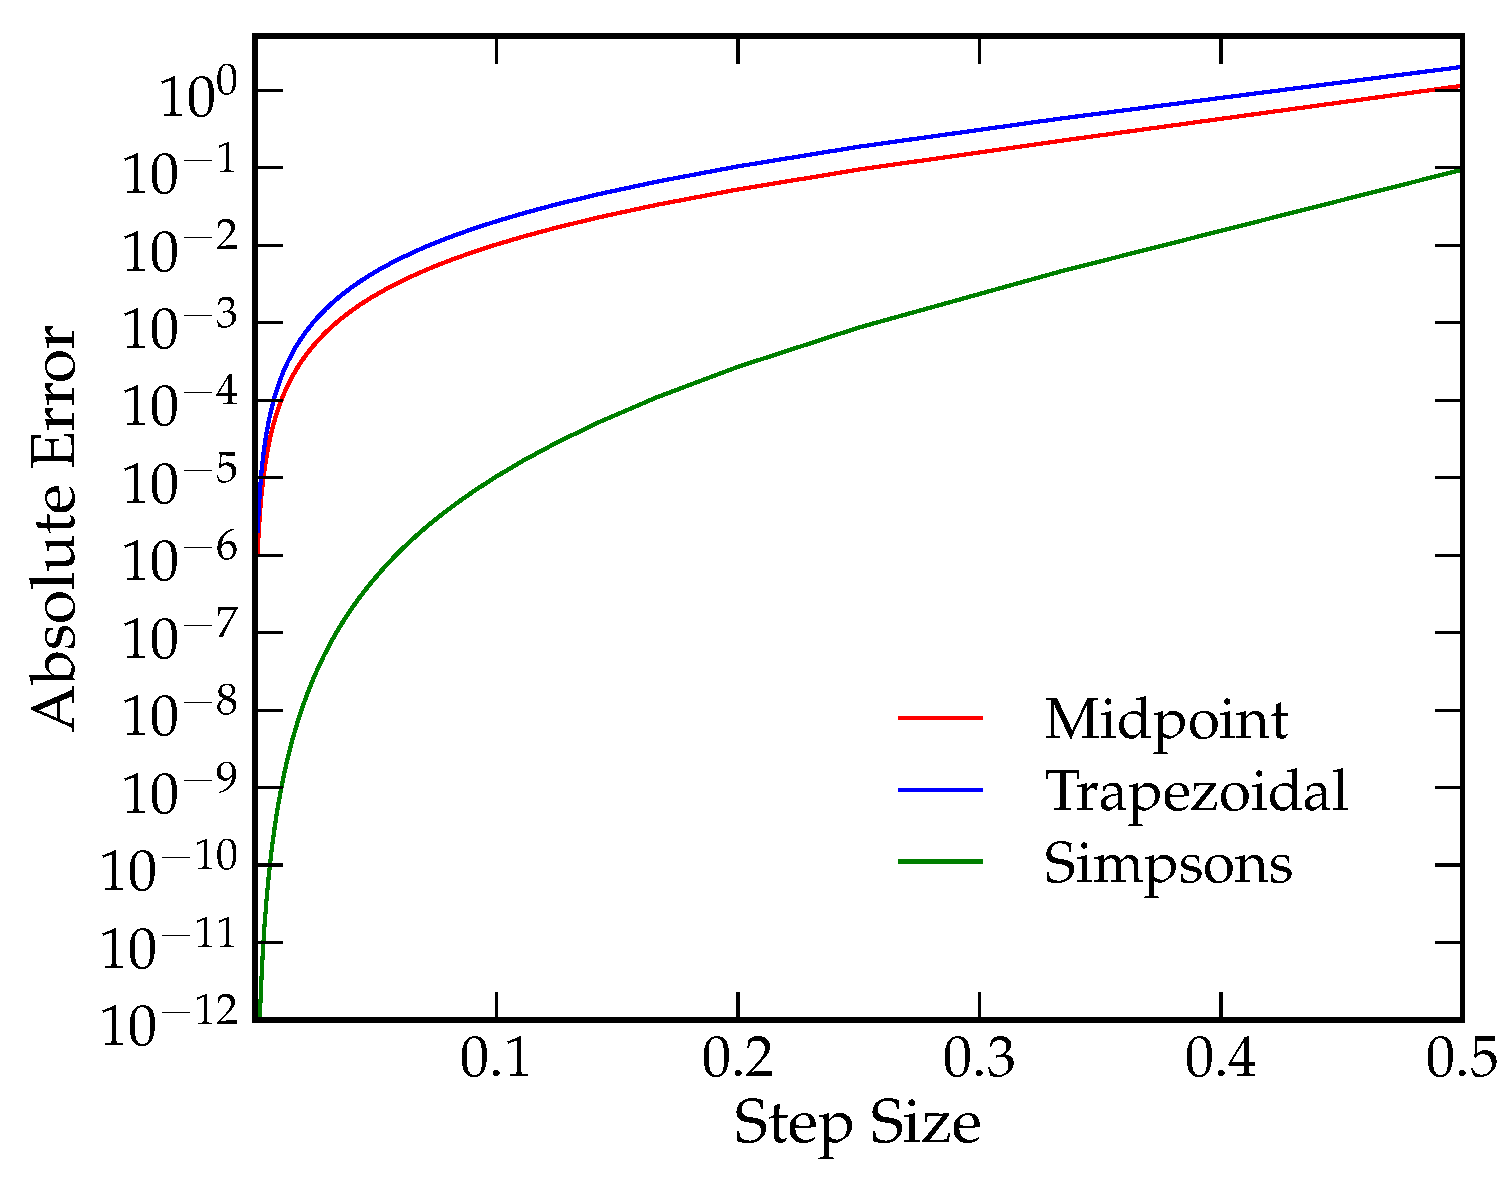
\includegraphics[width=0.5\textwidth]{1a.pdf}
\caption{For $sin(x)$ the Midpoint, Trapezoidal,
             and Simpsons rule all converge.}
\label{fig:sinx}
\end{figure}

\subsection{}

While we have shown that these methods converge for $sin(x)$ but this may be a 
fluke. We examine the function $x\ sin(x)$ in figure~\ref{fig:xsinx}. 

\begin{figure}[bth]
\centering
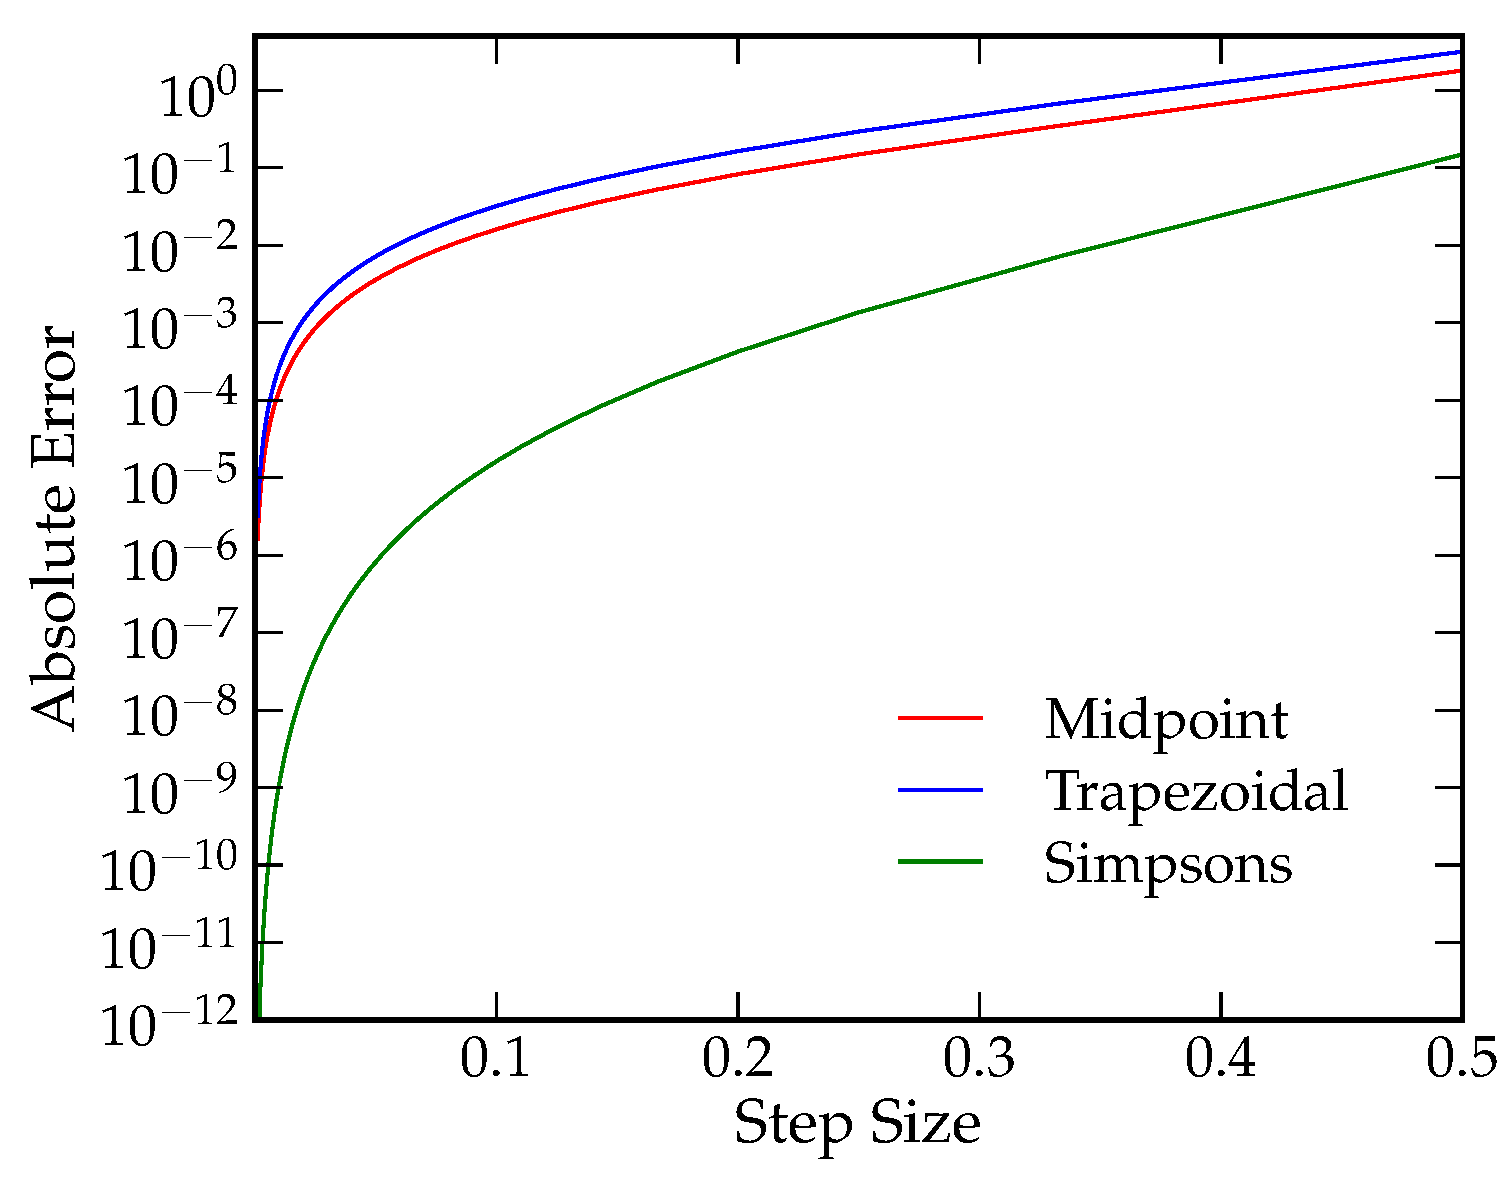
\includegraphics[width=0.5\textwidth]{1b.pdf}
\caption{For $x\ sin(x)$ the Midpoint, Trapezoidal, 
            and Simpsons rule all converge.}
\label{fig:xsinx}
\end{figure}

\section{Gaussian Quadrature}

When performing Gaussian-Laguerre quadrature the accuracy is determined by the
number of nodes that are used. To determine the convergance of the process
we take the Gaussian-Laguerre with the most nodes and treat that as the
'correct' answer. 

By subtracting it from the lower node estimations we get some determination of 
error. We can see from figure~\ref{fig:gauss_lag_error} that the error gets
exponentially smaller and thus can conlude that the Gaussian-Laguerre method
does infact converge. It does converge to the value of $1.52\ 10 ^{37}$ when we 
include the constant $\frac{8\pi(k_b T)^3}{(2 \pi \hbar c)^3}$

\begin{figure}[bth]
\centering
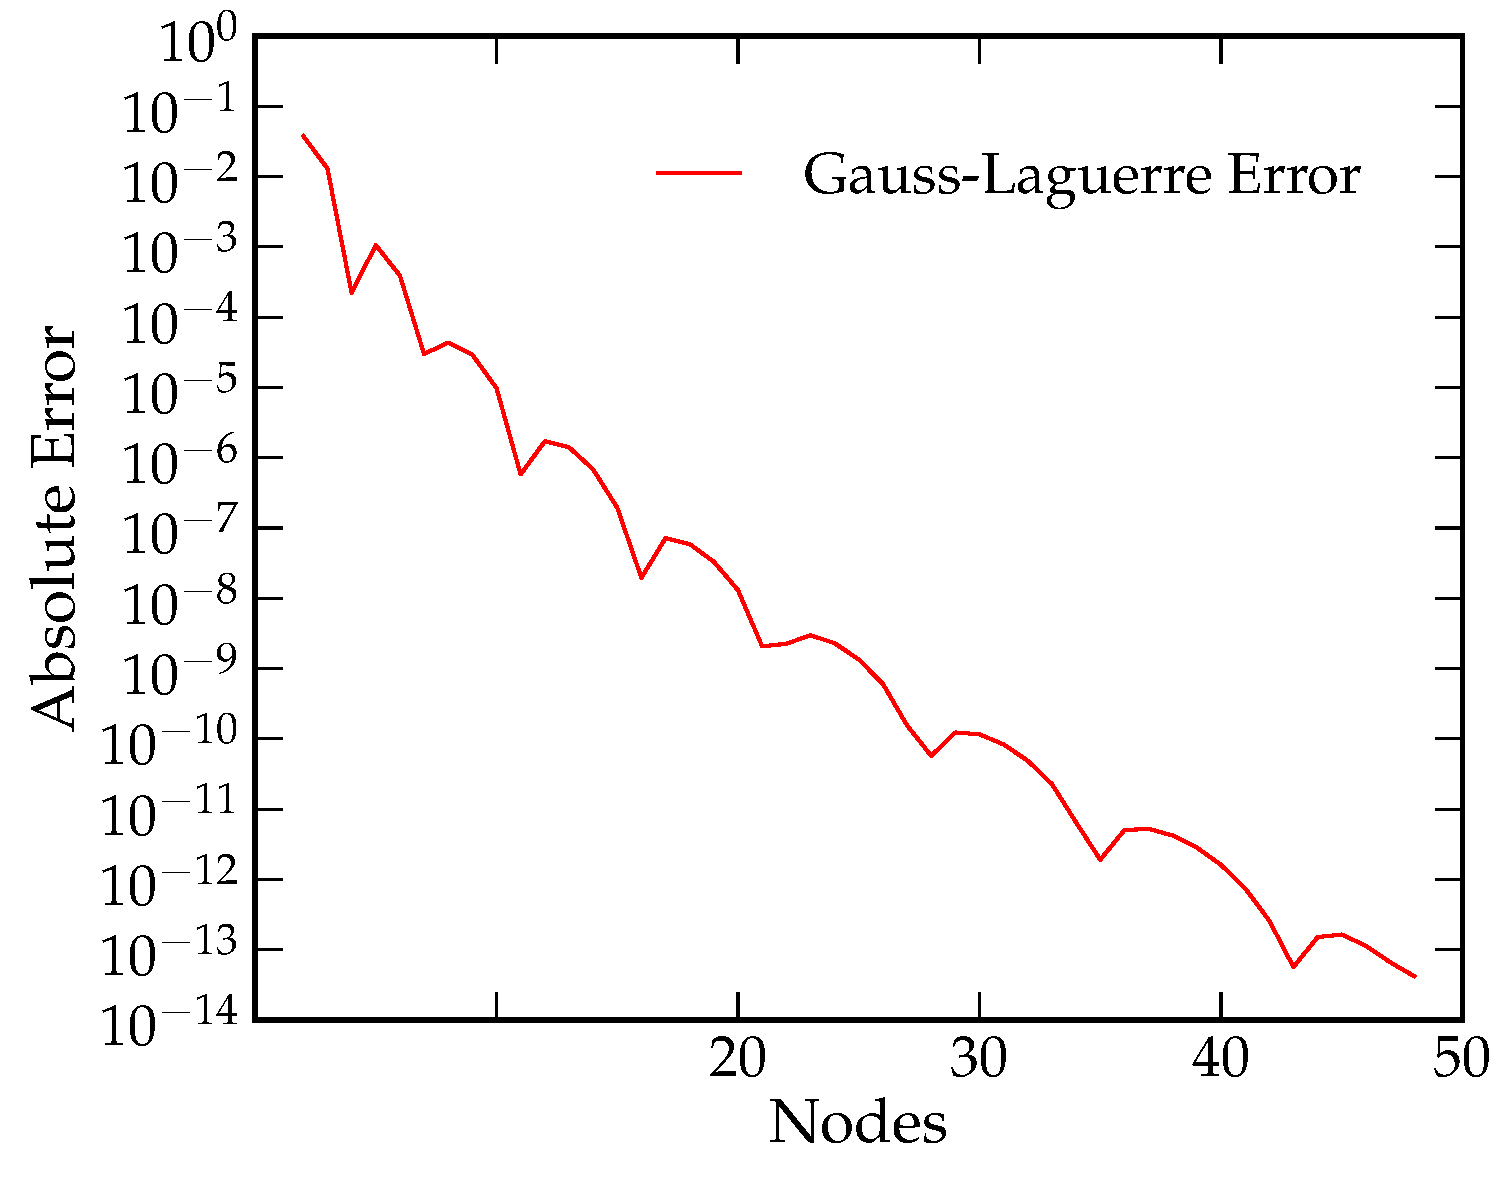
\includegraphics[width=0.5\textwidth]{2a.pdf}
\caption{Guass-Laguerre error convergance with increasing nodes.}
\label{fig:gauss_lag_error}
\end{figure}

\subsection{Gauss-Legendre Quadrature}

By binning the integral into segments and then utilizing the
Gaussian-Lagendre integration on each bin we can calculate an estimation of a
derivative of $n_e$. Note that when we sum the derivative multiplied by the
bin size we recover the estimated value of $n_e$.

\begin{figure}[bth]
\centering
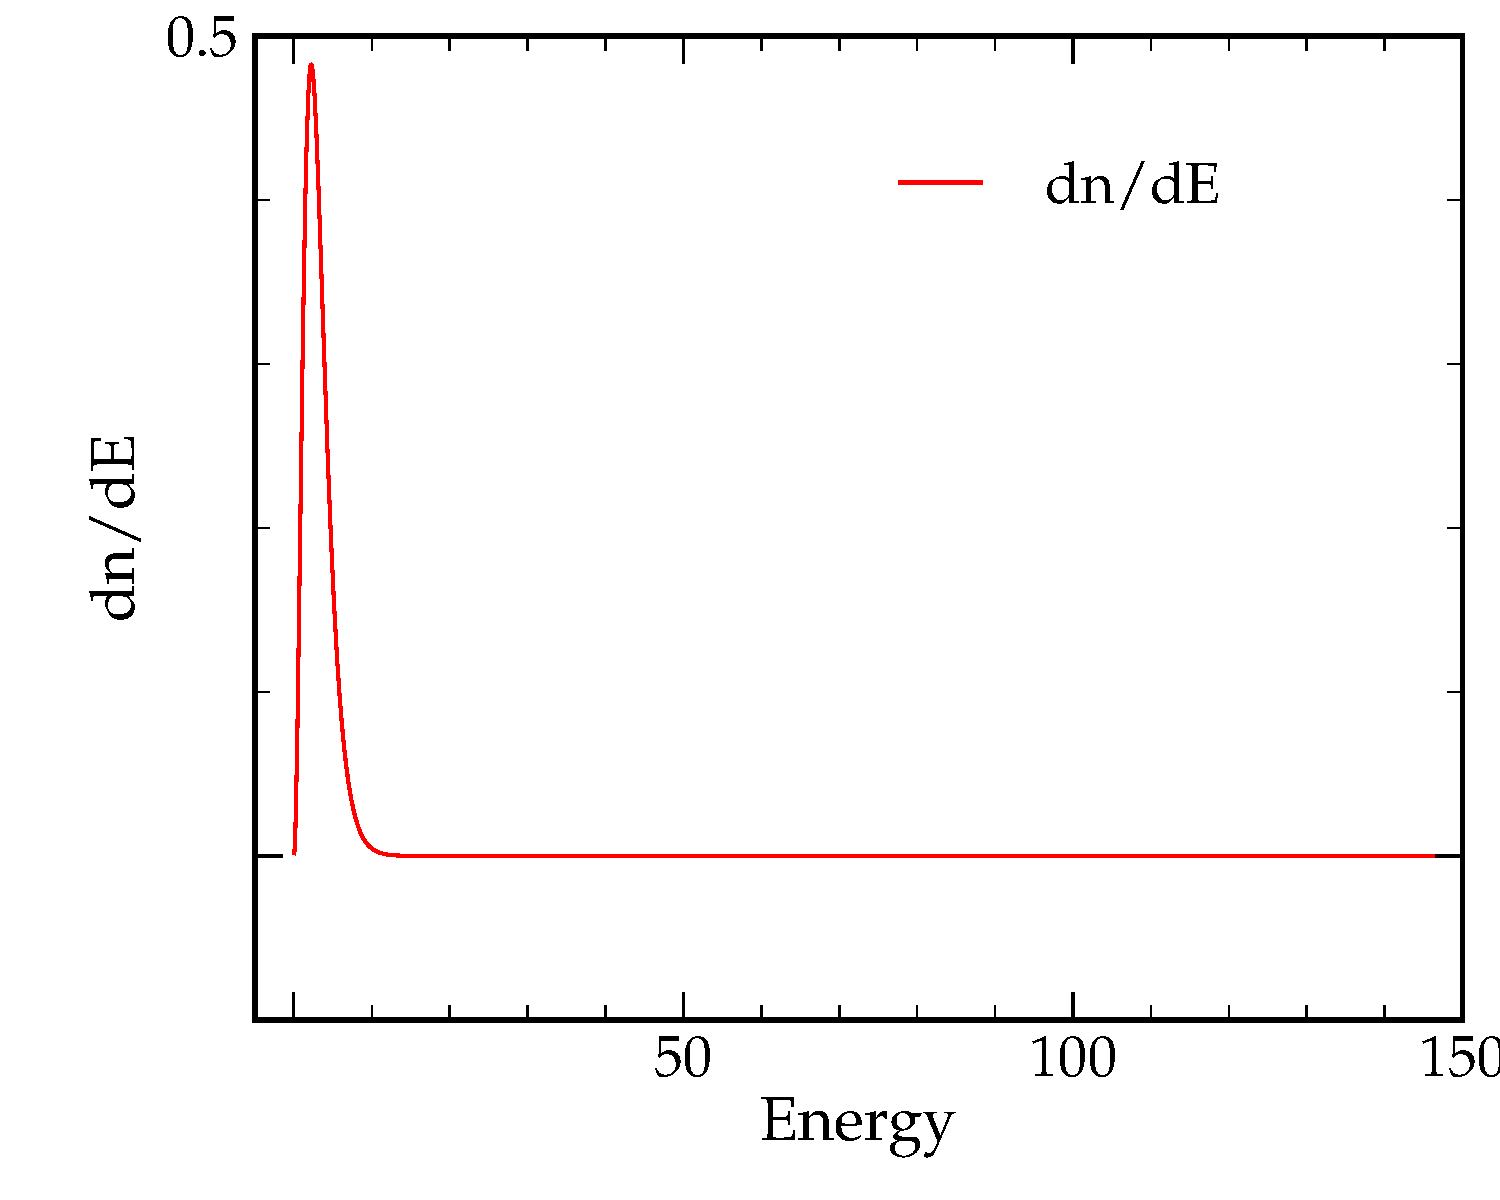
\includegraphics[width=0.5\textwidth]{2b.pdf}
\caption{Estimation of the derivative of $n_e$ using the Gaussian-Lagendre
           integration.}
\label{fig:dne}
\end{figure}

\end{document}




